
\documentclass[professionalfont]{beamer}

\usepackage{graphicx}
\usepackage{tabularx}
\usepackage[british]{datetime2}
\usetheme{default}
\usecolortheme{seagull}
\usepackage{newtxtext}
\setbeamertemplate{navigation symbols}{} % No navigation symbols
\definecolor{ntnu}{cmyk}{100,75,0,5}
%\setbeamercolor{alerted text}{fg=ntnu}
%\setbeamercolor{frame title}{fg=black}
%\setbeamercolor{title}{fg=black}
%\setbeamercolor{subtitle}{fg=black}
%\setbeamercolor{section in head/foot}{fg=black} % Not working
%\setbeamercovered{transparent}

\setbeamertemplate{itemize item}{\color{white}$\bullet$} 
% Include above line to remove bullet indicators

\setbeamertemplate{footline}{
\begin{tabularx}{\textwidth} {
	 >{\raggedright\arraybackslash}X 
  	 >{\centering\arraybackslash}X 
  	 >{\centering\arraybackslash}X 
  	 >{\centering\arraybackslash}X 
  	 >{\centering\arraybackslash}X 
  	 >{\centering\arraybackslash}X}
	
	\insertshortauthor & 
	\insertshorttitle &
	\insertdate &
	\insertsection &
	$\big|$ \insertframenumber /\inserttotalframenumber
\end{tabularx}
}

\makeatletter
\makeatother

%----------------------------------------------------------------------------------------
%	TITLE PAGE
%----------------------------------------------------------------------------------------

\title[Trial Lecture]{The Effects of Slavery and Colonialism on Contemporary
African Politics}

\subtitle{Trial Lecture}

\author[Wishman]{Marius Swane Wishman} 
\date{\today} 
\institute{NTNU}

\begin{document}

\begin{frame}[plain]
\titlepage 
\end{frame}

\section{Introduction} 

\begin{frame}{This lecture will cover}
\begin{itemize}
	\item The slave trade 
\begin{itemize}
	\item[-] Scope and effects 
\end{itemize}
	\item Colonialism 
		\begin{itemize}
			\item[-] Effects on the number of states 
			\item[-] Local and national level effects 
			
		\end{itemize}
	\item Outcomes (dependent variables)
		\begin{itemize}
			\item[-] Conflict
			\item[-] Economic development
			\item[-] Democracy
		\end{itemize}
\end{itemize}	
\end{frame}

\section{The Slave Trade}

\begin{frame}{The African slave trade(s)}

\begin{figure}
	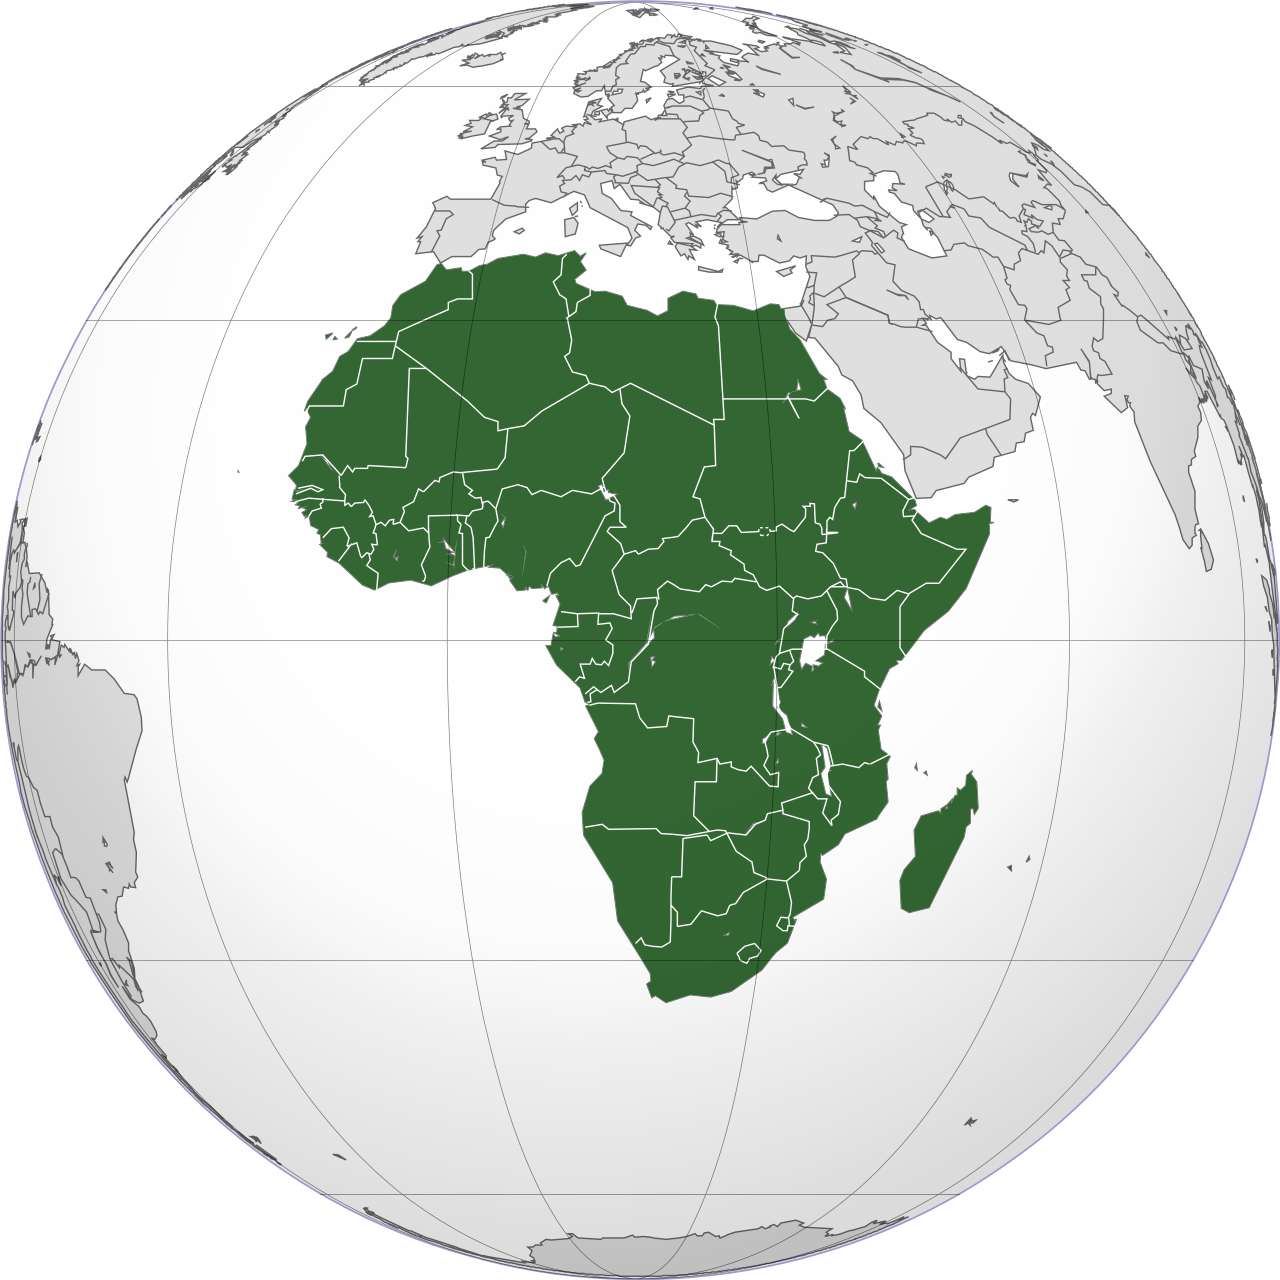
\includegraphics[width=.7\linewidth]{img/africa.png}
\end{figure}

\end{frame}

\section{Colonialism}

\begin{frame}
	\centering 
	\begin{Large}
		Colonialism
	\end{Large}
\end{frame}

\begin{frame}
	\begin{figure}
		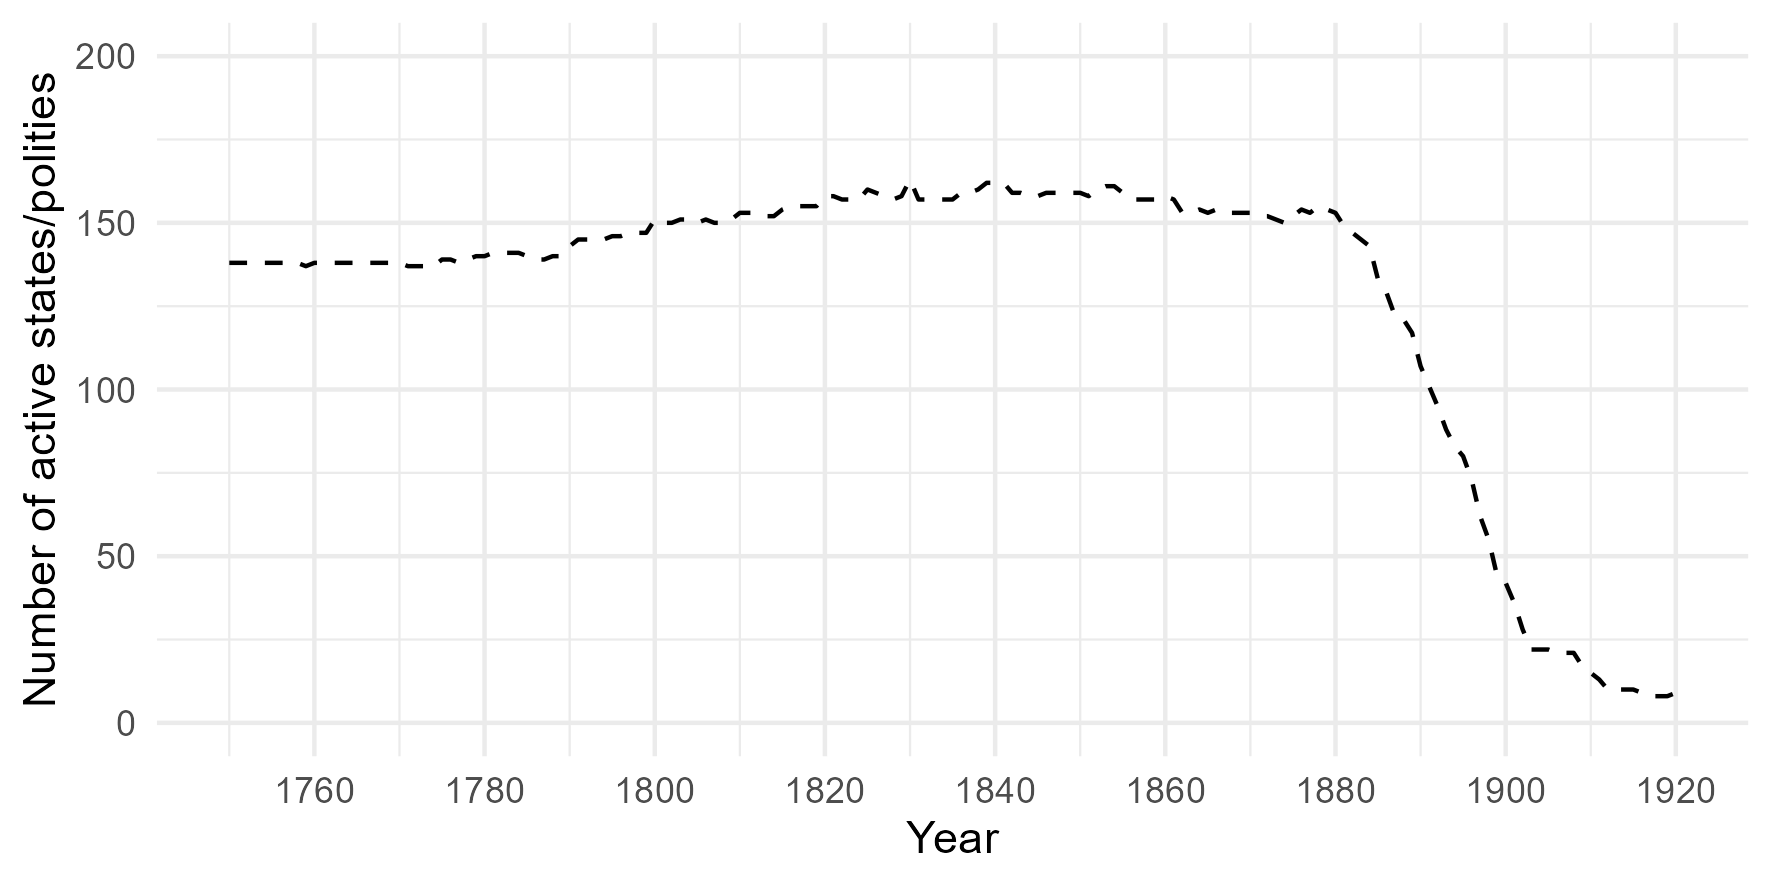
\includegraphics[width=\linewidth]{img/N_States_Only_Over_Time.png}
	\end{figure}
\end{frame}

\begin{frame}
	\begin{figure}
		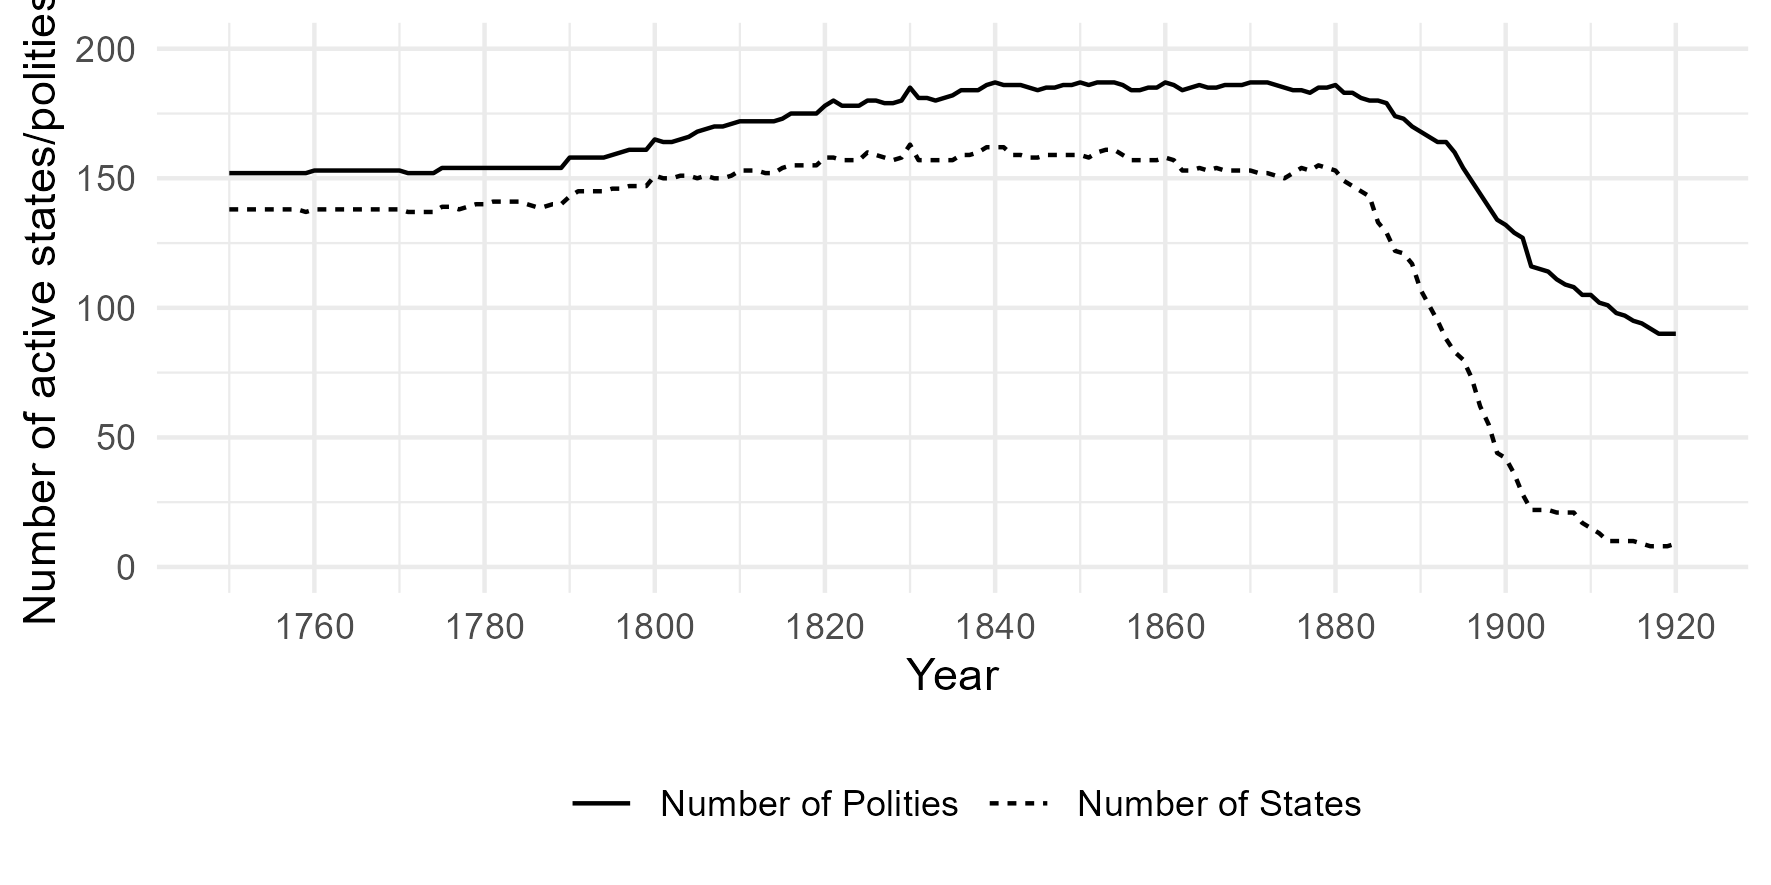
\includegraphics[width=\textwidth]{img/N_States_Over_Time.png}
	\end{figure}
\end{frame}

\section{Conclusion}

\begin{frame}{Conclusion}
	\begin{table}
	\begin{tabularx}{\textwidth}{>{\centering\arraybackslash}X>{\centering\arraybackslash}X>{\centering\arraybackslash}X}
		\textbf{The slave trade} & & \\
					 & $\rightarrow$ Ethnic fractionalization & $\rightarrow$ Conflict (?) \& Retarded economic
		development \\	
					 & $\rightarrow$ Retarded political development (with
		some exceptions) & $\rightarrow$ Retarded economic development \\
		\textbf{Colonialism} & & \\
				     & $\rightarrow$ Conflict & \\
			& Retarded economic development & \\
			& $\rightarrow$ Democracy (demand for/seeds of) \\
	\end{tabularx}
	\end{table}
\end{frame}

\end{document}
